\subsection{Controller}
%
%\begin{frame}{Controller}{}
%
%  \begin{block}{PID}
%
%  \end{block}
%  
%  \begin{block}{Tunning}
%
%  \end{block}
%
%  \begin{block}{Comparion}
%
%  \end{block}
%
%\end{frame}

%Overview
\begin{frame}{Modelling}{Moving Angle System}
  \begin{block}{Moving Angle System:}

	  \begin{itemize}
  	  	\item Servomotor
	  	\item Gear
	  	\item Sensor
	  	\item Controller
	  \end{itemize}

	  \begin{figure}
        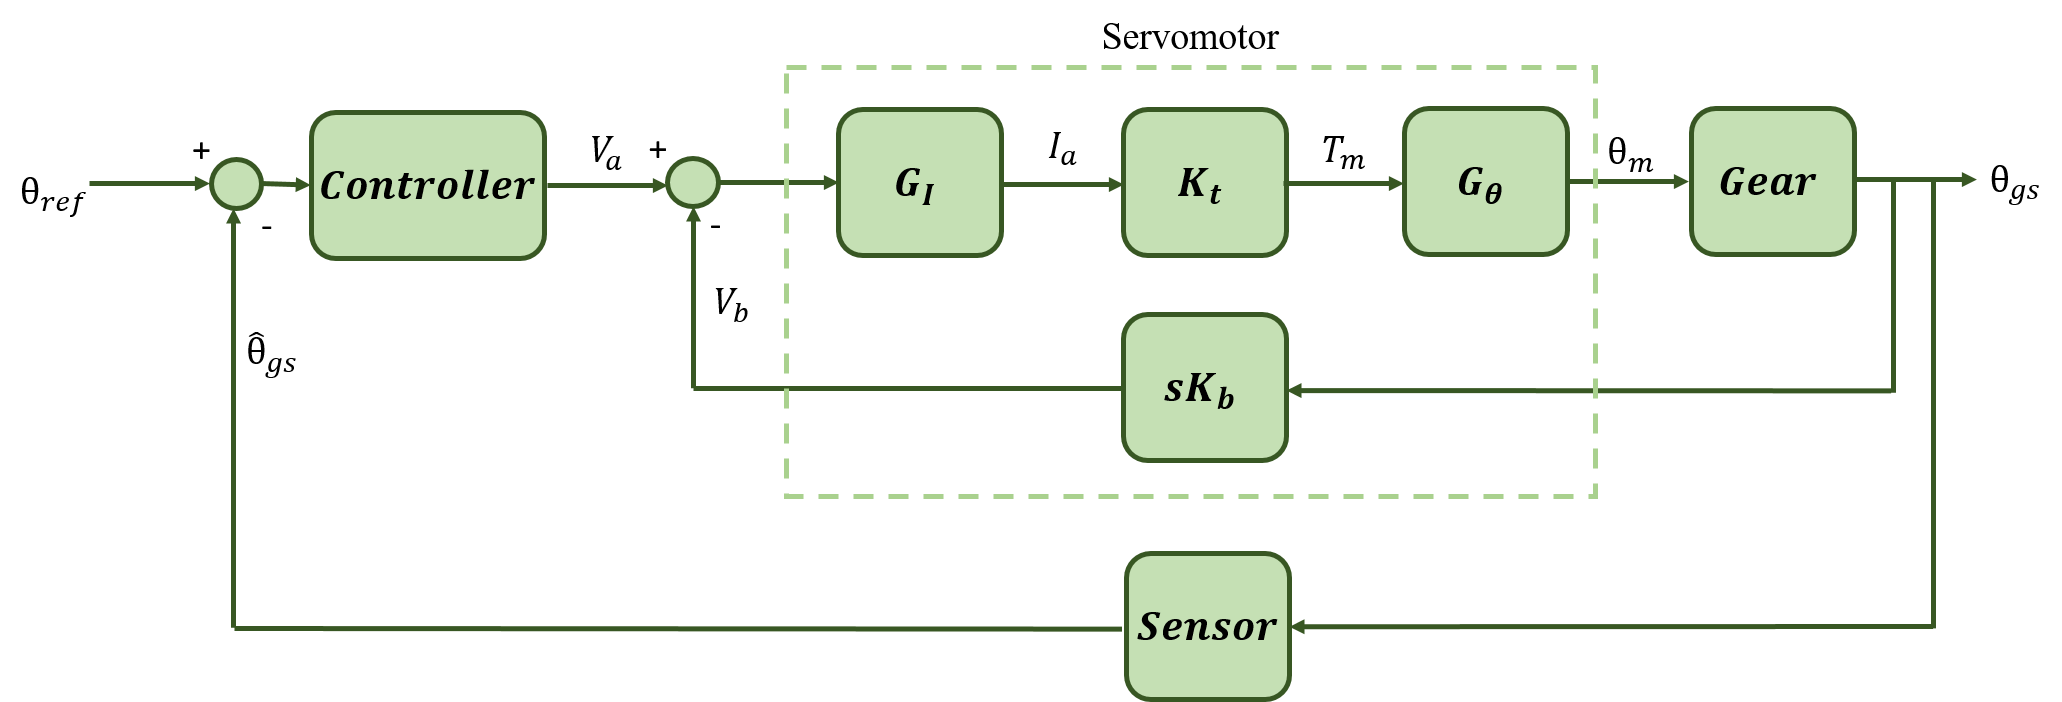
\includegraphics[scale=0.26]{../report/figures/servo+gear+noise.png}
      \end{figure}
  
  \end{block}
\end{frame}


%Servomotor
\begin{frame}{Modelling}{Moving Angle System}
  \begin{block}{Moving Angle System:}

	  \begin{itemize}
	  	\item Servomotor
	  \end{itemize}

	  \begin{figure}
        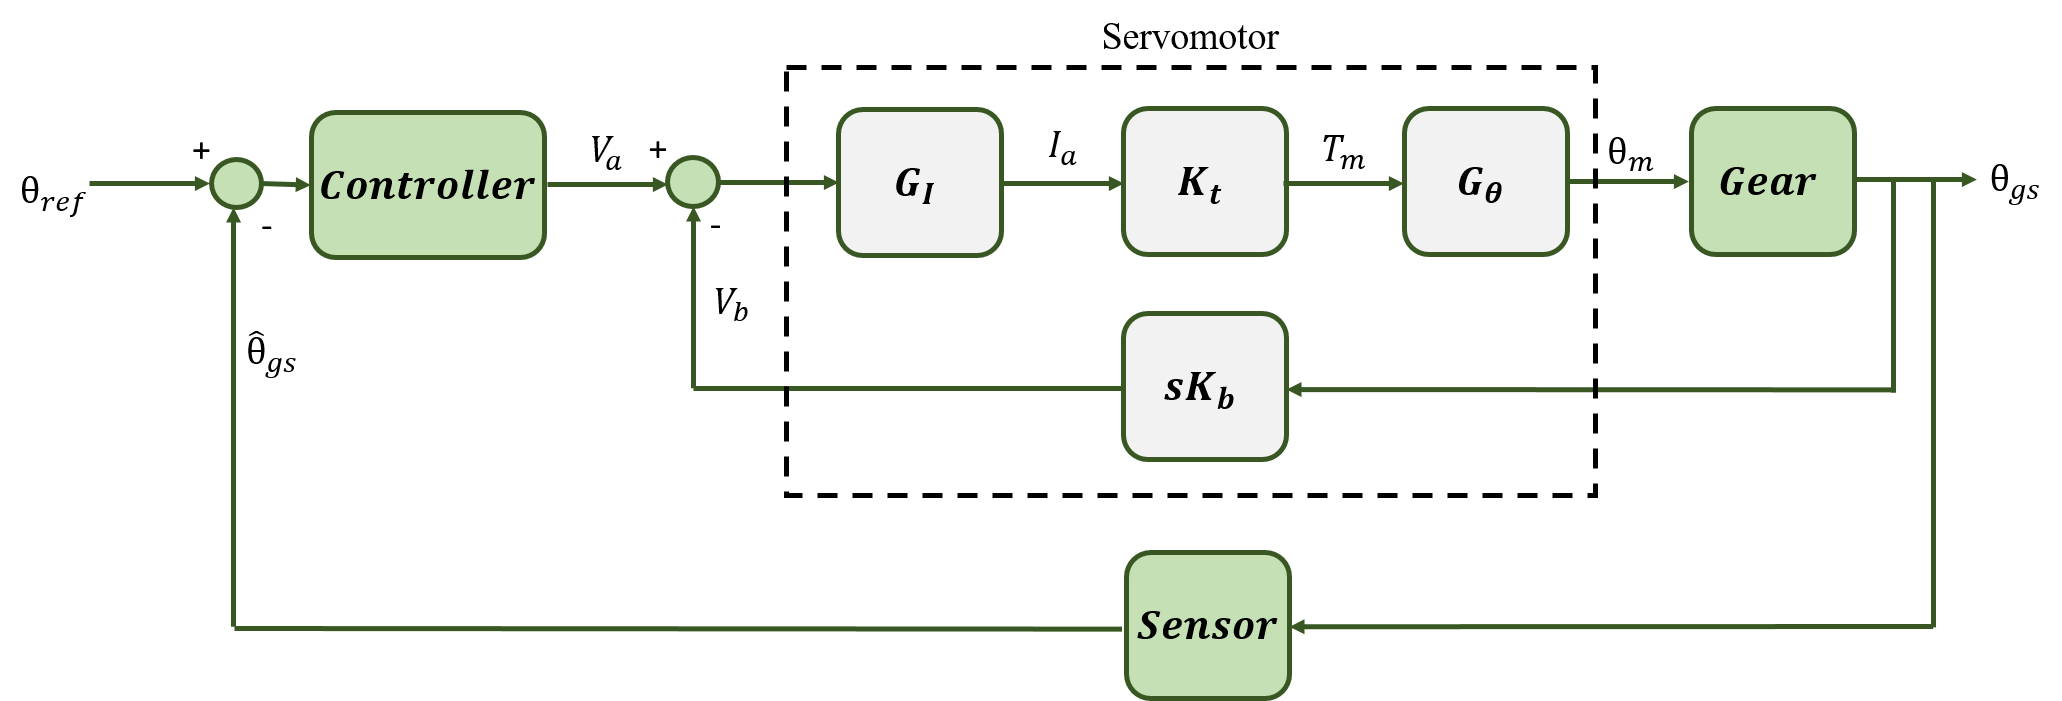
\includegraphics[scale=0.26]{../report/figures/servo+gear+noise+servomotor.png}
      \end{figure}
  
  \end{block}
\end{frame}

%Gear
\begin{frame}{Modelling}{Moving Angle System}
  \begin{block}{Moving Angle System:}
	  \begin{itemize}
	  	\item Gear
	  \end{itemize}
	  \begin{figure}
        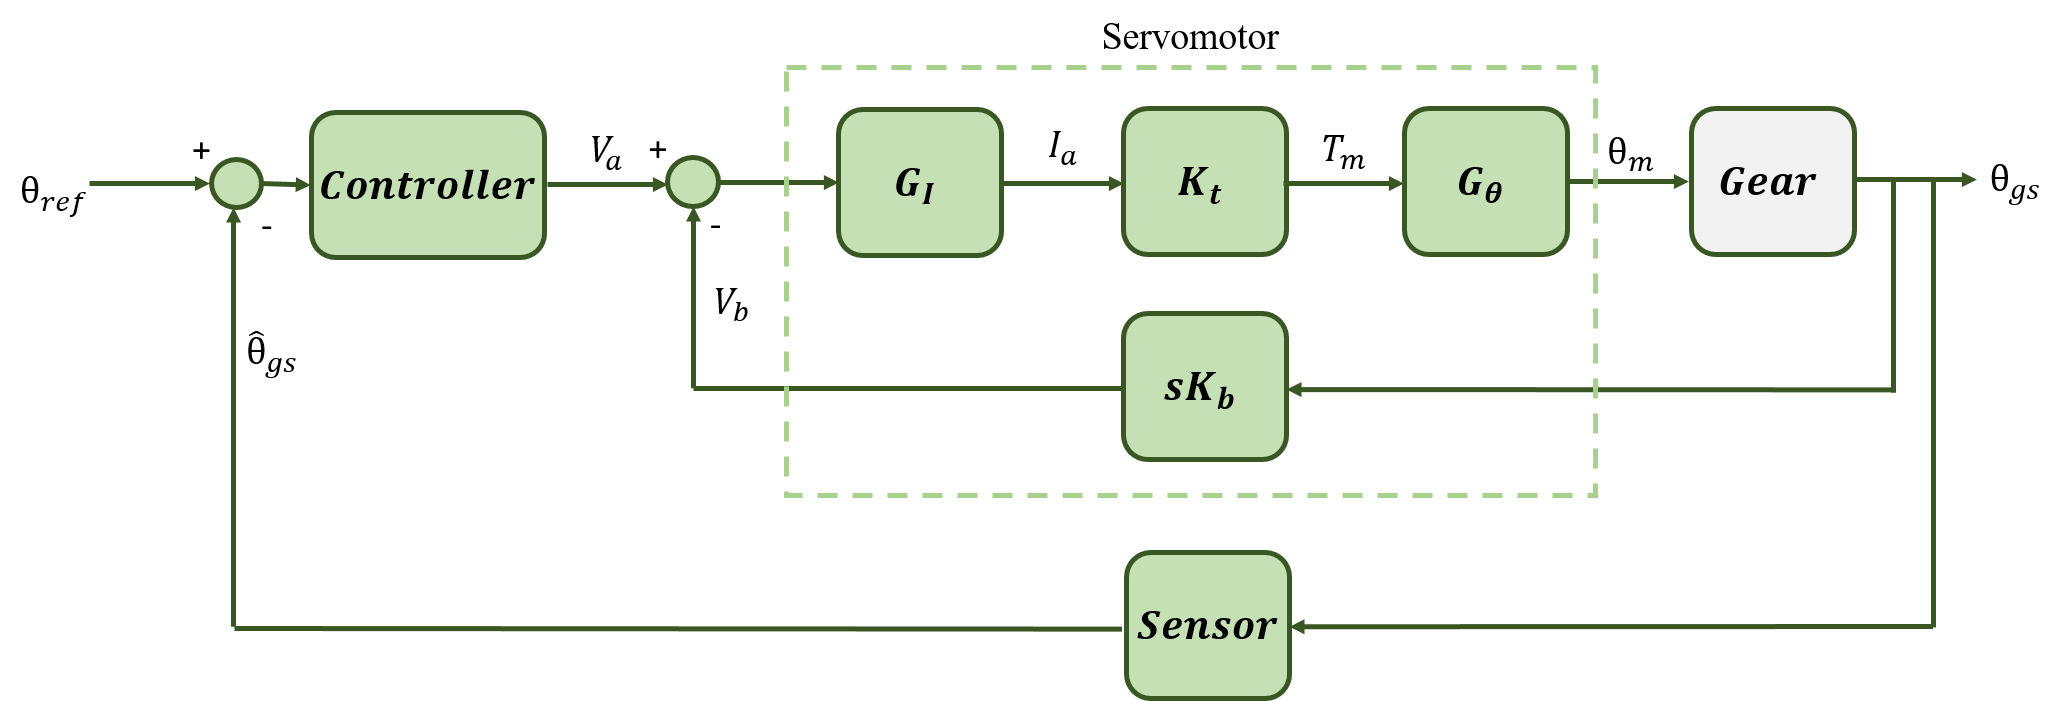
\includegraphics[scale=0.26]{../report/figures/servo+gear+noise+gear.png}
      \end{figure}  
  \end{block}
\end{frame}

%Sensor
\begin{frame}{Modelling}{Moving Angle System}
  \begin{block}{Moving Angle System:}

	  \begin{itemize}
	  	\item Sensor
	  \end{itemize}

	  \begin{figure}
        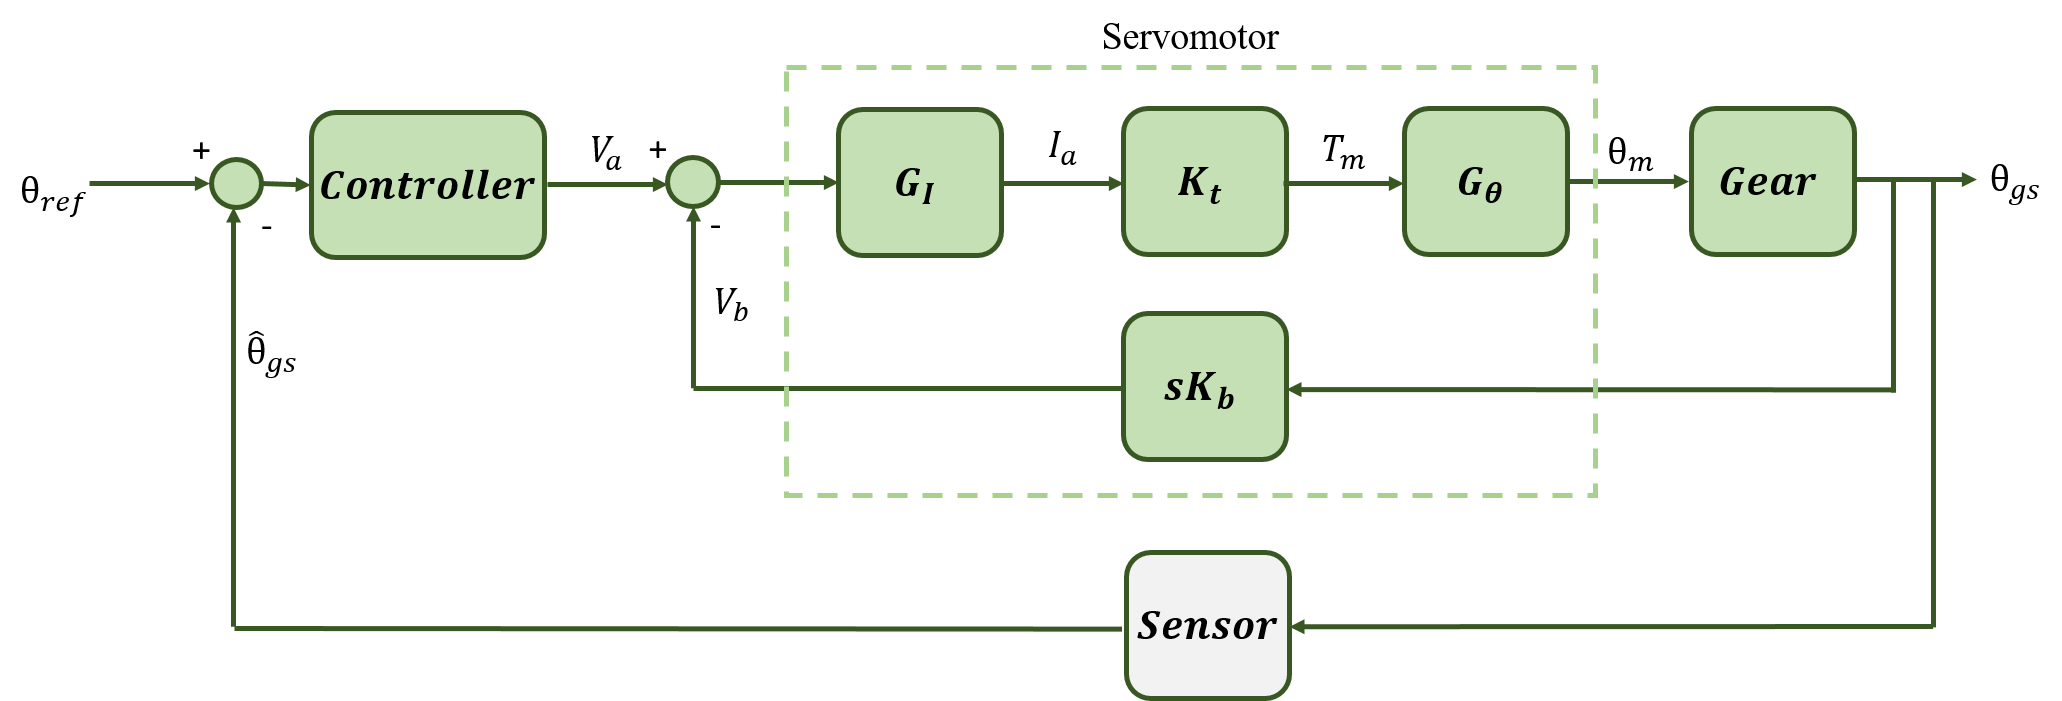
\includegraphics[scale=0.26]{../report/figures/servo+gear+noise+sensor.png}
      \end{figure}
  
  \end{block}
\end{frame}


%Controller
\begin{frame}{Modelling}{Moving Angle System}
  \begin{block}{Moving Angle System:}
	  \begin{itemize}
	  	\item Controller
	  \end{itemize}
	  \begin{figure}
        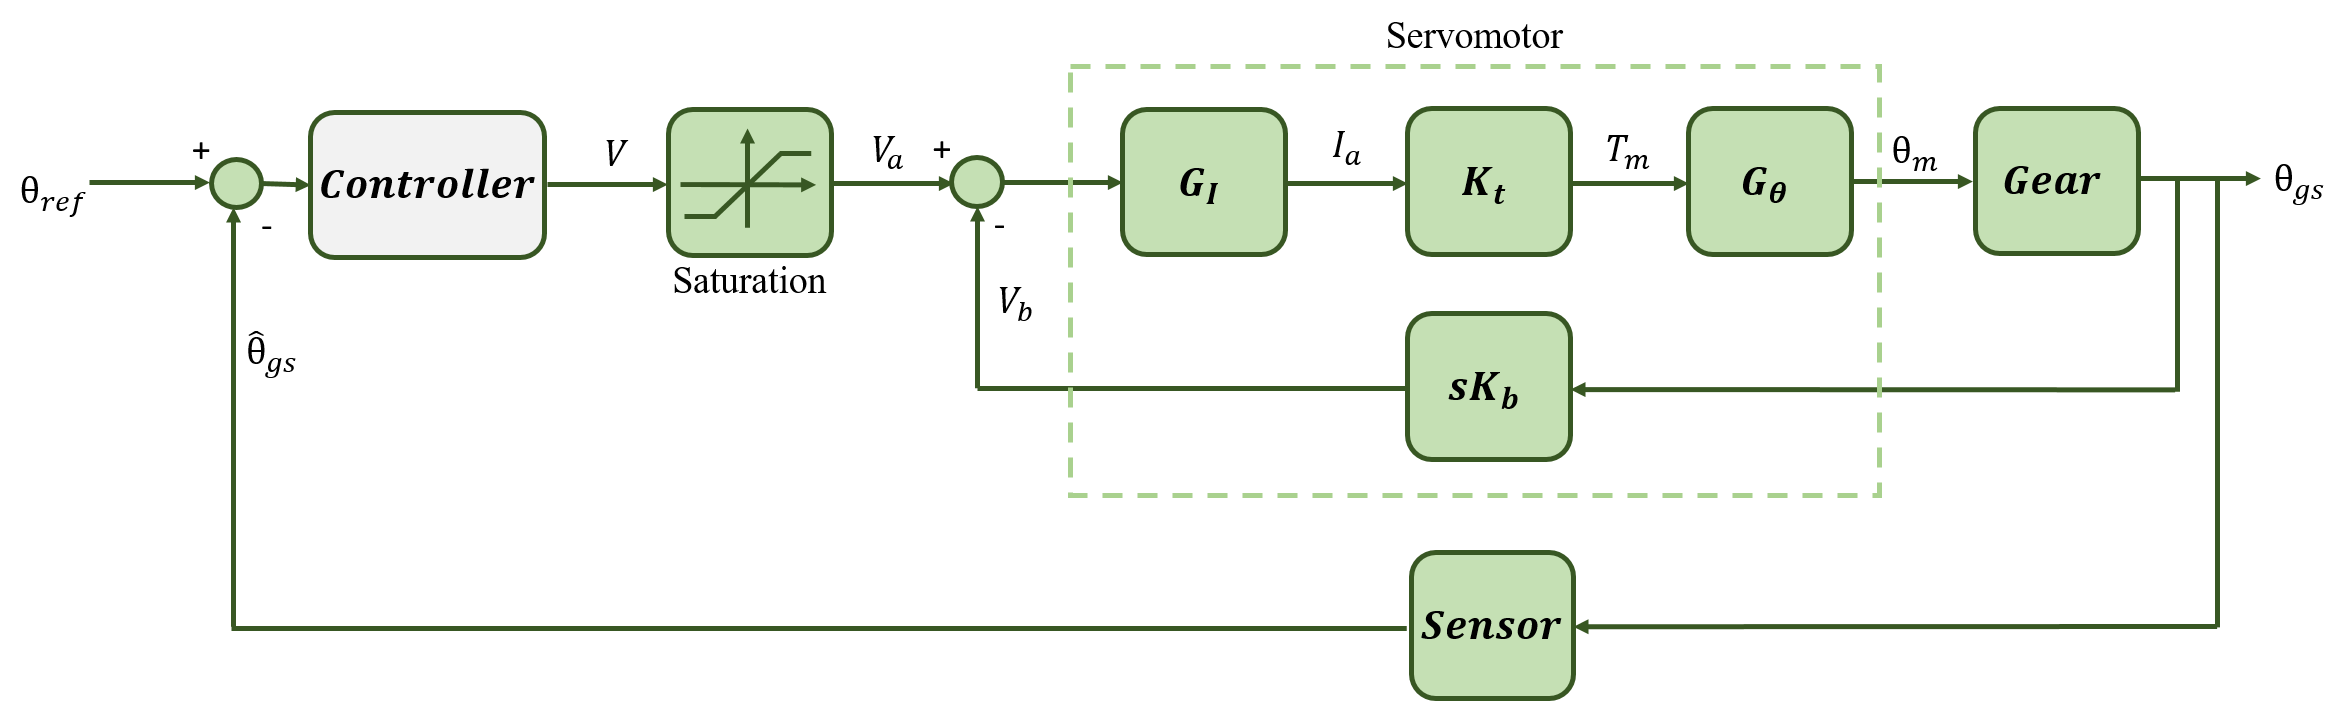
\includegraphics[scale=0.26]{../report/figures/servo+gear+noise+controller.png}
      \end{figure}
  \end{block}
\end{frame}


%%%
%%Controller
\begin{frame}{Controller}{What controllers}
  \begin{block}{Type of control:}

	  \begin{itemize}
	  	\item PID control
	 	\begin{itemize}
	  	\item Proportional
	  	\item Derivative
	  	\item Integral
	  	\item Combination of them
	  \end{itemize}
	  \end{itemize}


  \end{block}
\end{frame}

%%%  HOW DID WE DESIGN THE CONTROLLERS?
%%Controller
\begin{frame}{Controller}{Tuning Method}
  \begin{block}{Good Gain Method:}
	  \begin{enumerate}
	  	\item Ti = $\infty$, Td = 0, Kp = 1
	  	\item Increase Kp until finding a slight overshoot
		\item Ti = 1.5$\cdot T_{out}$
		\item Td = $\frac{Ti}{4}$
	  \end{enumerate}
	  
  \end{block}
\end{frame}

%%Tuning Method
\begin{frame}{Controller}{Tuning Methods}
  \begin{block}{Good Gain Method}
  
	  \begin{enumerate}
	  	\item Ti = $\infty$, Td = 0, Kp = 1
	  \end{enumerate}
	  \begin{figure}
       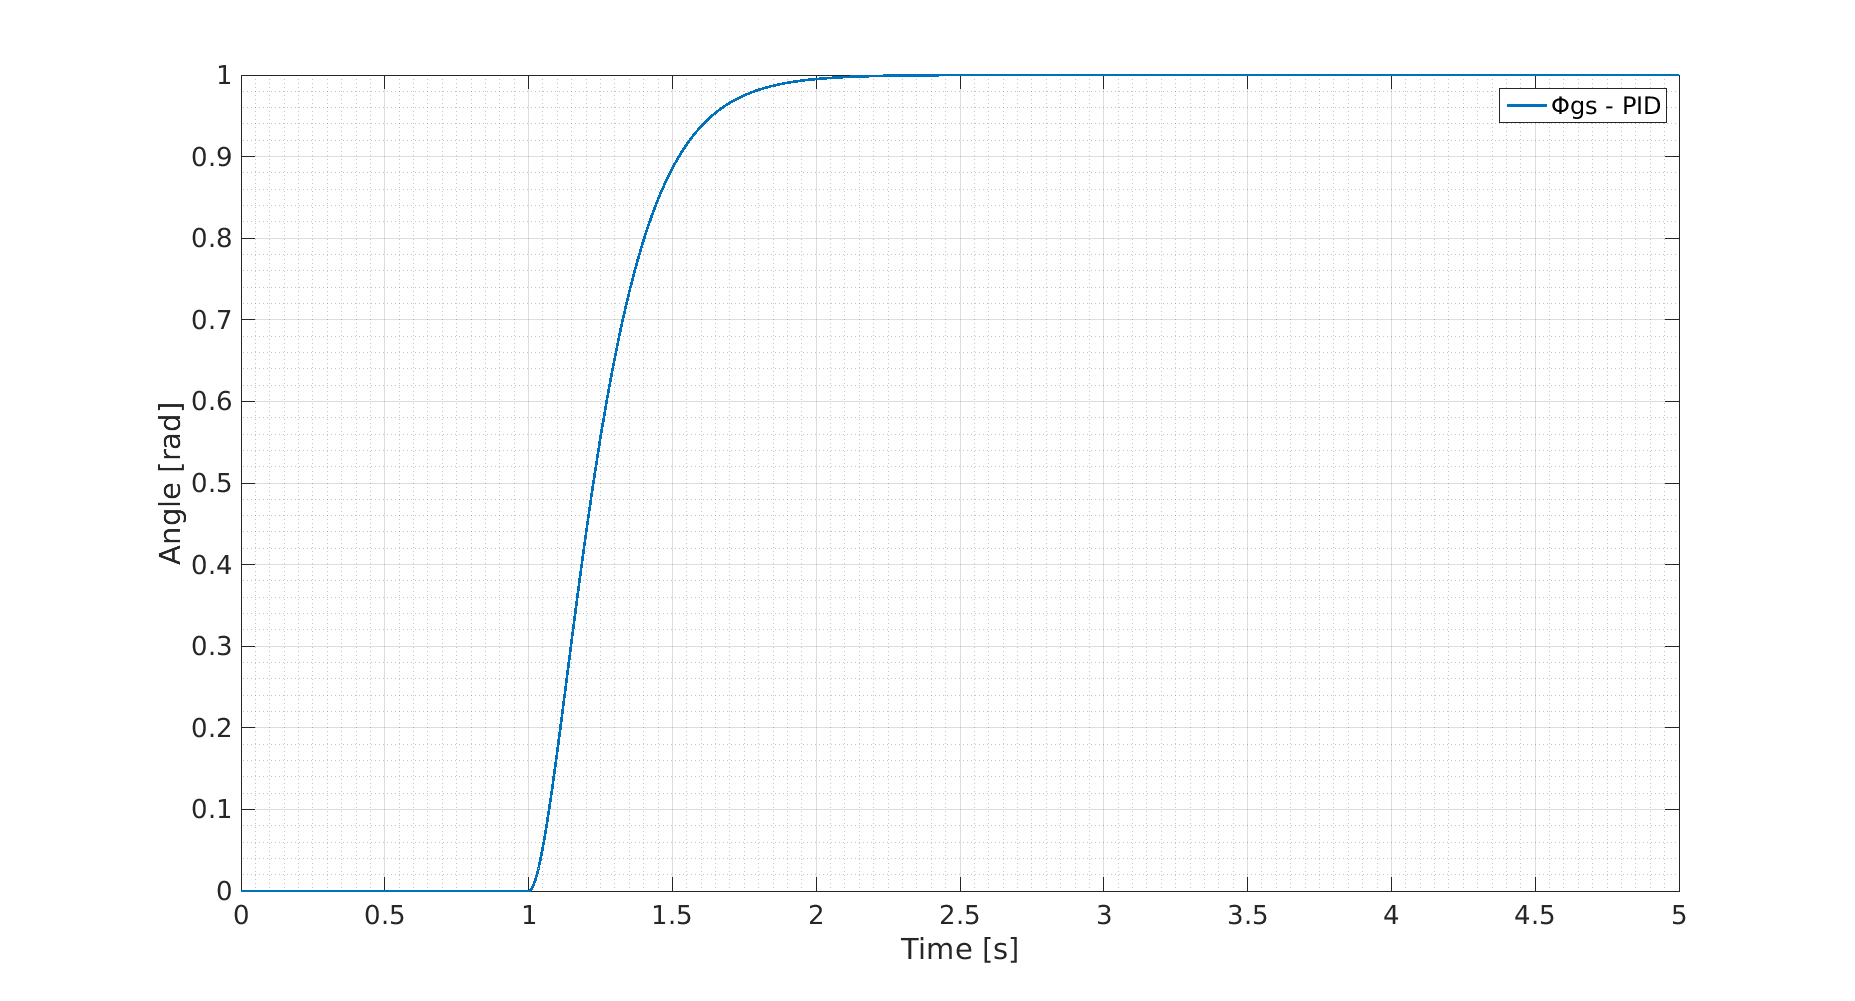
\includegraphics[scale=0.20]{../report/figures/GG1.png}
      \end{figure}
  
  \end{block}
\end{frame}

%Tuning Method
\begin{frame}{Controller}{Tuning Methods}
  \begin{block}{Good Gain Method}
  
	  \begin{enumerate}
	  \setcounter{enumi}{1}
	  	\item Increase Kp until finding a slight overshoot and well damped
	  	\begin{itemize}
	  	\item Save $T_{out}$ = Time between overshoot and undershoot
	  	\end{itemize}
	  \end{enumerate}
	  \begin{figure}
       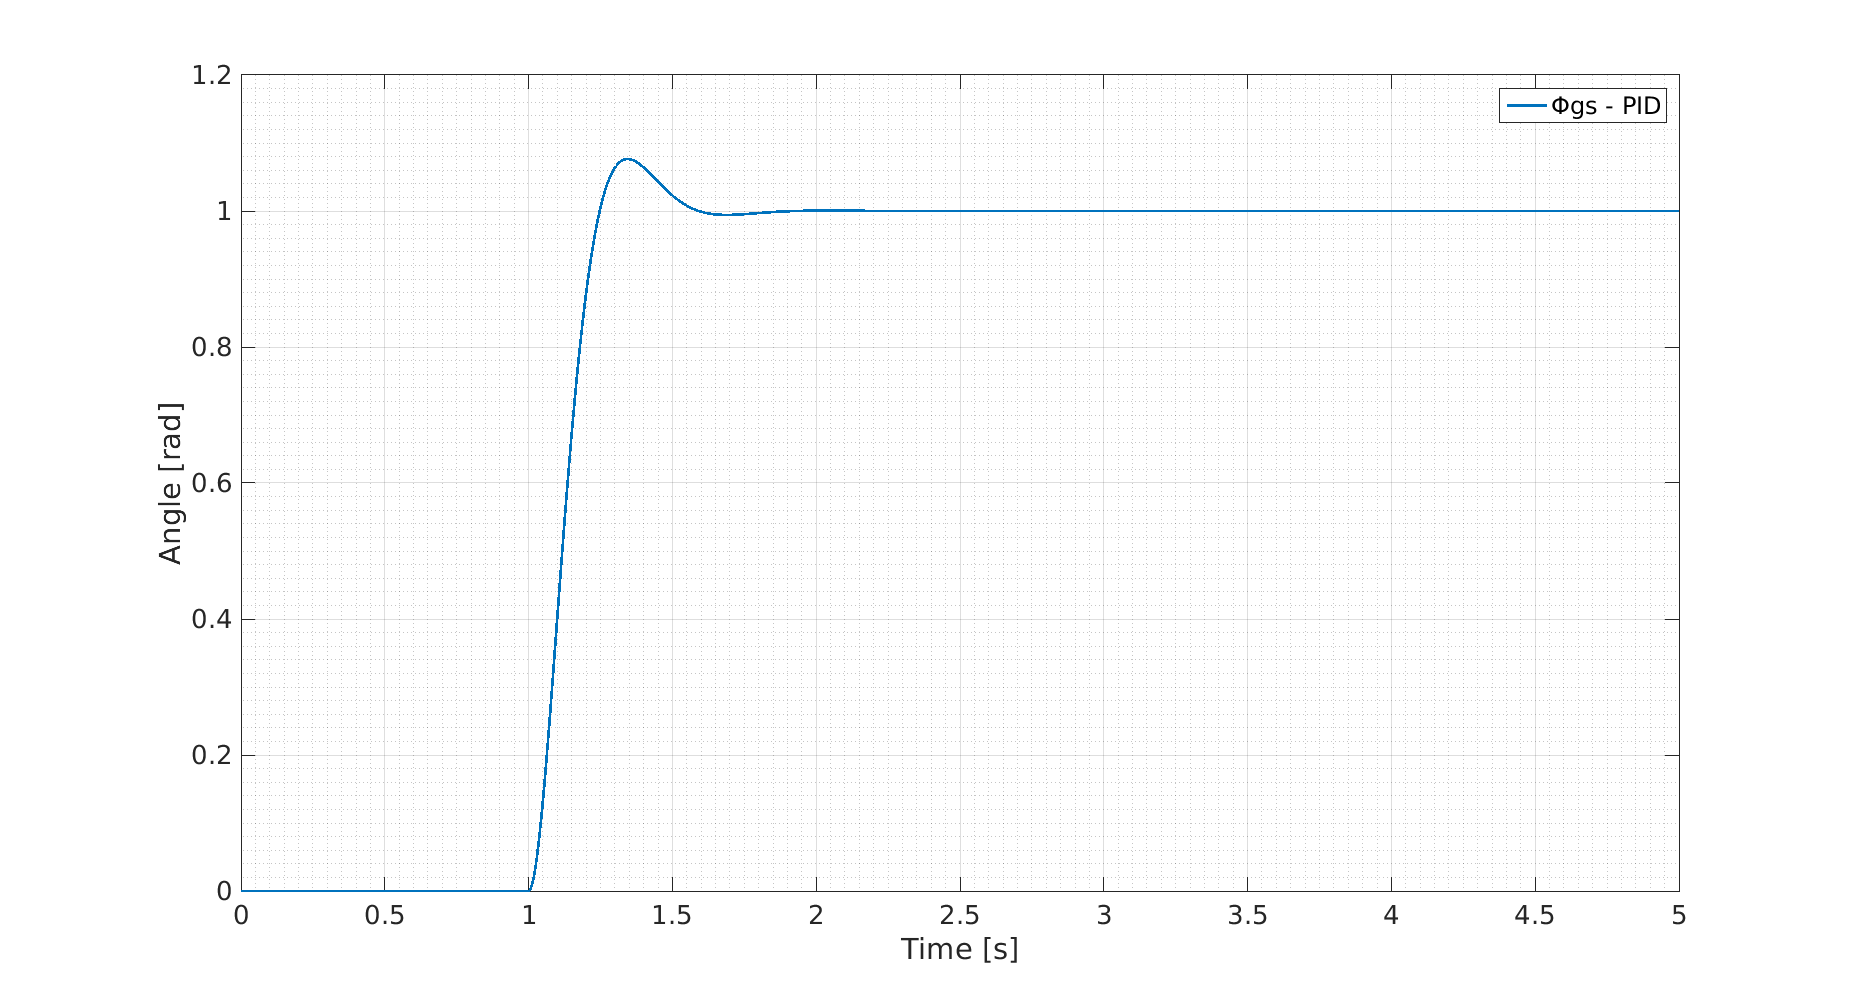
\includegraphics[scale=0.18]{../report/figures/GG2.png}
      \end{figure}
  
  \end{block}
\end{frame}

%Tuning Method
\begin{frame}{Controller}{Tuning Methods}
  \begin{block}{Good Gain Method}
  
	  \begin{enumerate}
	  \setcounter{enumi}{2}
	  	\item Ti = 1.5$\cdot T_{out}$
	  \end{enumerate}
	  \begin{figure}
       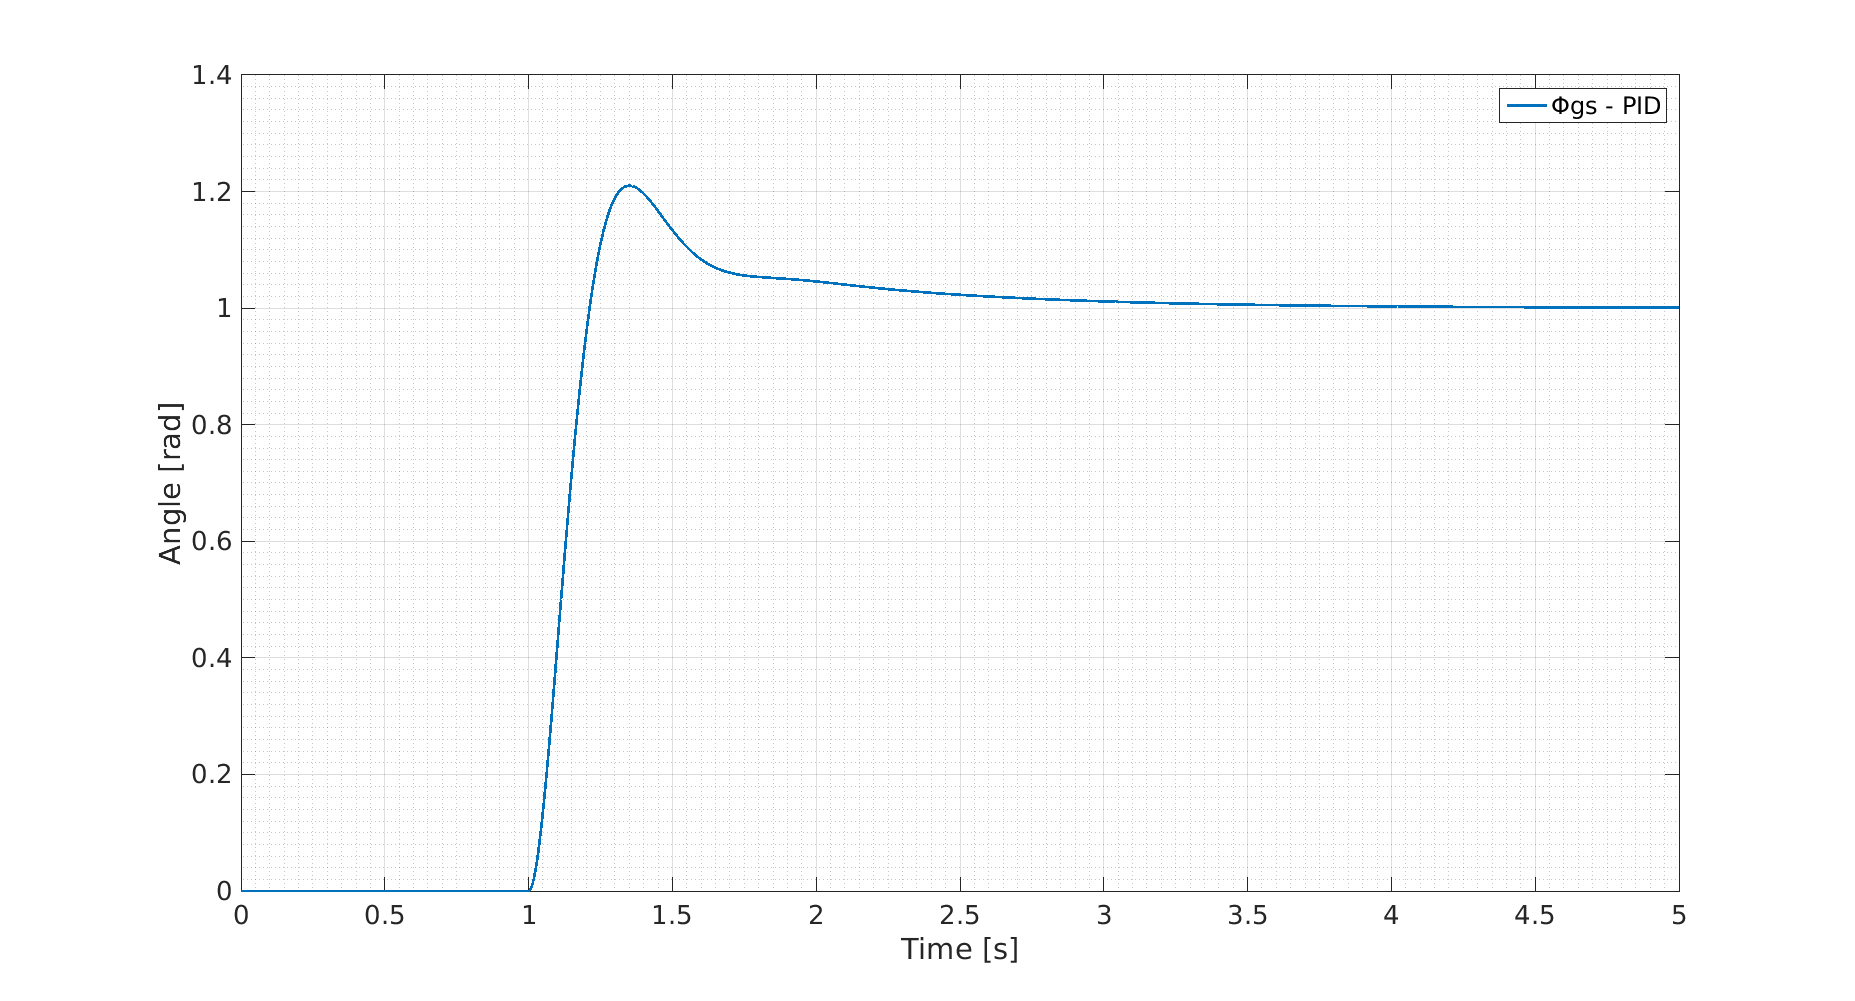
\includegraphics[scale=0.20]{../report/figures/GG3.png}
      \end{figure}
  
  \end{block}
\end{frame}



%Tuning Method
\begin{frame}{Controller}{Tuning Methods}
  \begin{block}{Good Gain Method}
  
	  \begin{enumerate}
	  \setcounter{enumi}{3}
	  	\item Td = $\frac{Ti}{4}$
	  \end{enumerate}
	  \begin{figure}
       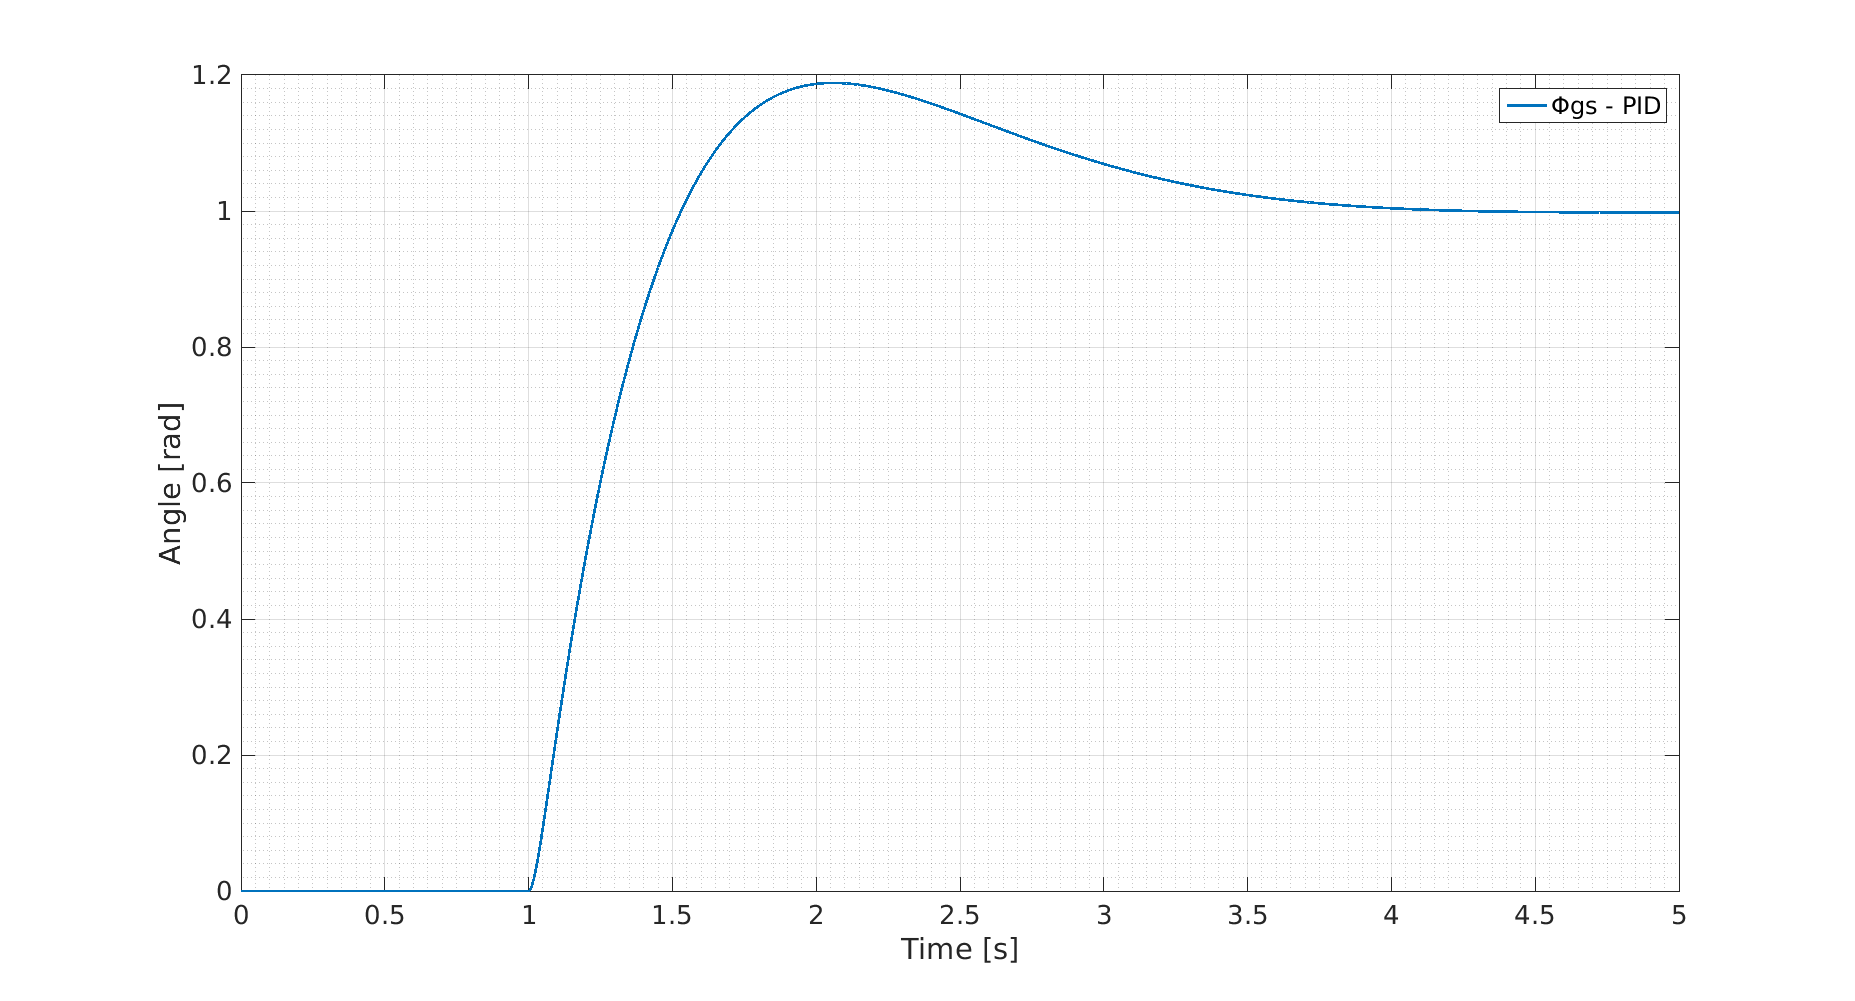
\includegraphics[scale=0.20]{../report/figures/GG4.png}
      \end{figure}
  
  \end{block}
\end{frame}


%Tuning Method
\begin{frame}{Controller}{Tuning Methods}
  \begin{block}{Good Gain Method}
  
	 \begin{itemize}
	  	\item Disadvantages:
	  \begin{itemize}
	  	\item Time consuming
	  	\item A lot of steps
	  	\begin{itemize}
	  	\item Uncertainties of the different steps	  	
	  	\end{itemize}

	  \end{itemize}
	\end{itemize}
  
  \end{block}
\end{frame}


%%Controller
\begin{frame}{Controller}{Tuning method}
  \begin{block}{PID Simulink Box}

	  \begin{itemize}
	  \item Advantages:
	  \begin{itemize}
	  	\item Automatic Tuning Tool
	  	\item Easier to design multiple controllers
	  	\item Adjust different parameters  	
	  \end{itemize}
	  \end{itemize}

  \end{block}
\end{frame}

%Comparison
\begin{frame}{Controller}{Comparison of step responses}
  \begin{block}{Different controllers:}
  
	  \begin{itemize}
	  	\item PI and PID - highest overshoot
	  		  \begin{itemize}
	  			\item 0.16rad and 0.19rad
	  			\item 9.17deg and 10.8deg
	  			\end{itemize}
	  	\item P and PD - no overshoot, shorter settling time, but still steady state error
	  \end{itemize}

	  \begin{figure}
        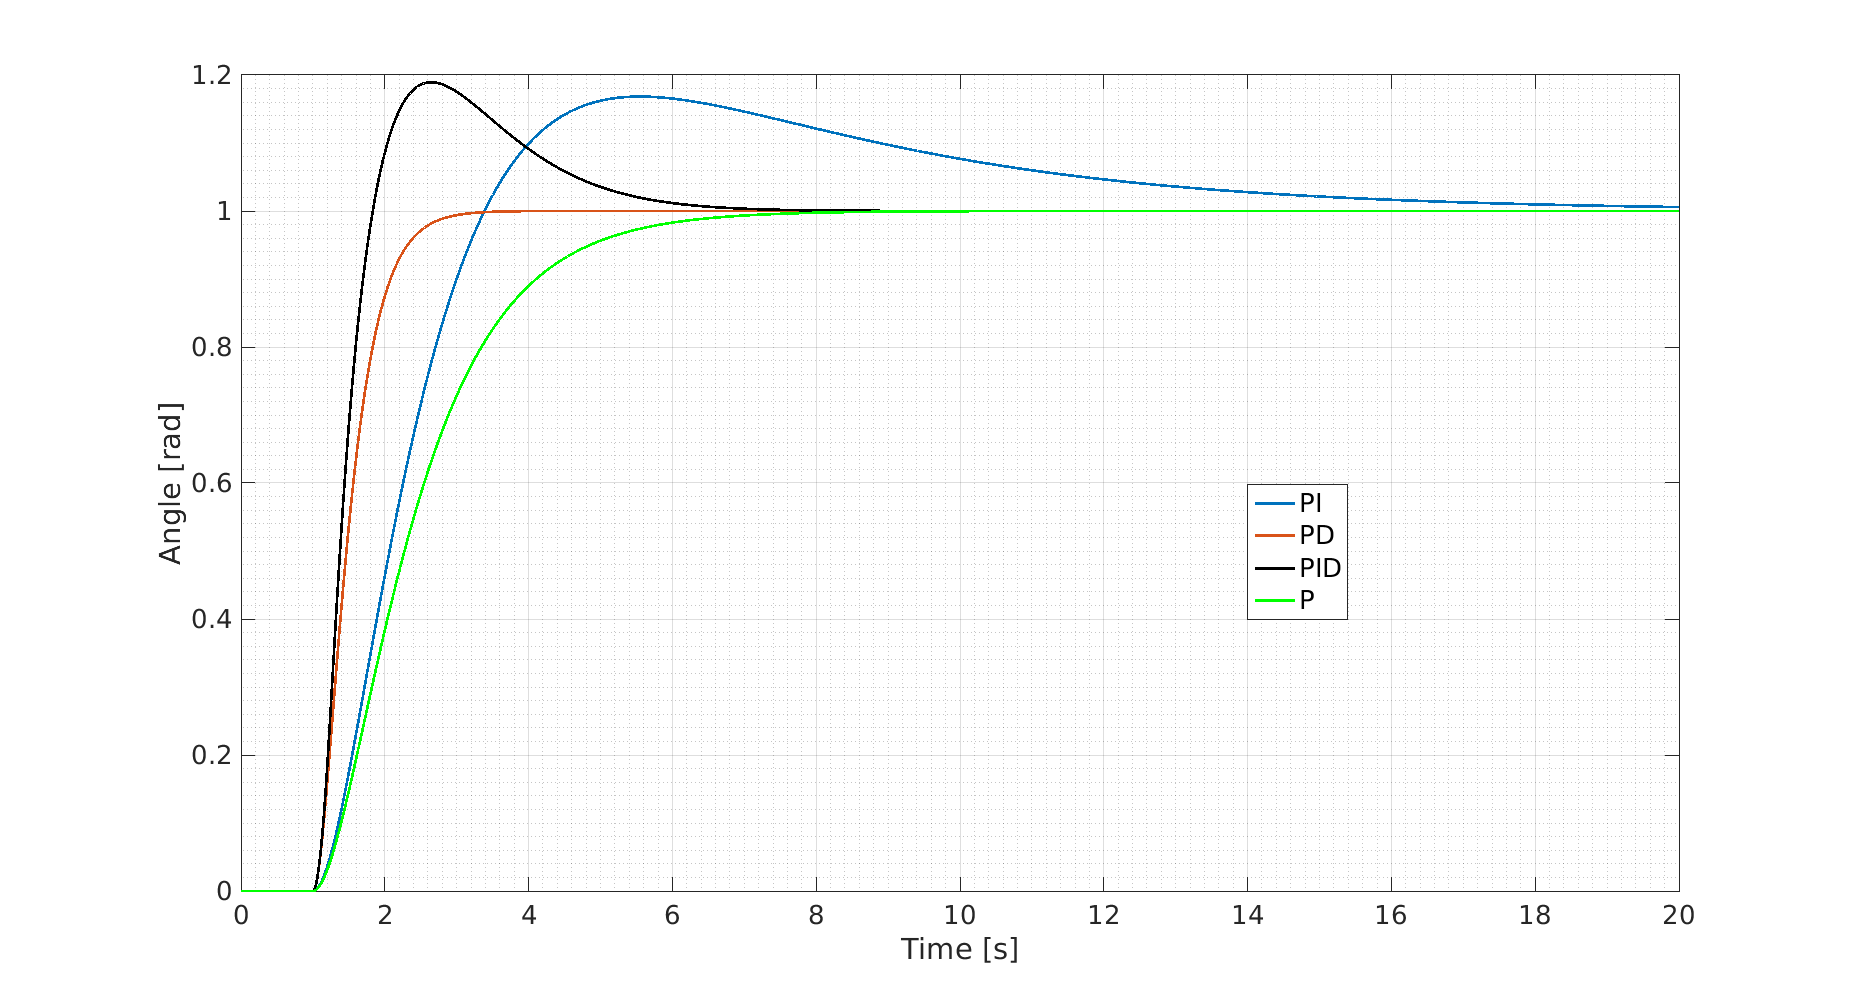
\includegraphics[scale=0.15]{../report/figures/full_comp.png}
      \end{figure}
  
  \end{block}
\end{frame}

%Comparison
\begin{frame}{Controller}{Comparison of step responses}
  \begin{block}{Different controllers with noise:}

	  \begin{itemize}
	  	\item P faster than PD
	  	\item P reacts more to noise then PD
	  \end{itemize}

	  \begin{figure}
        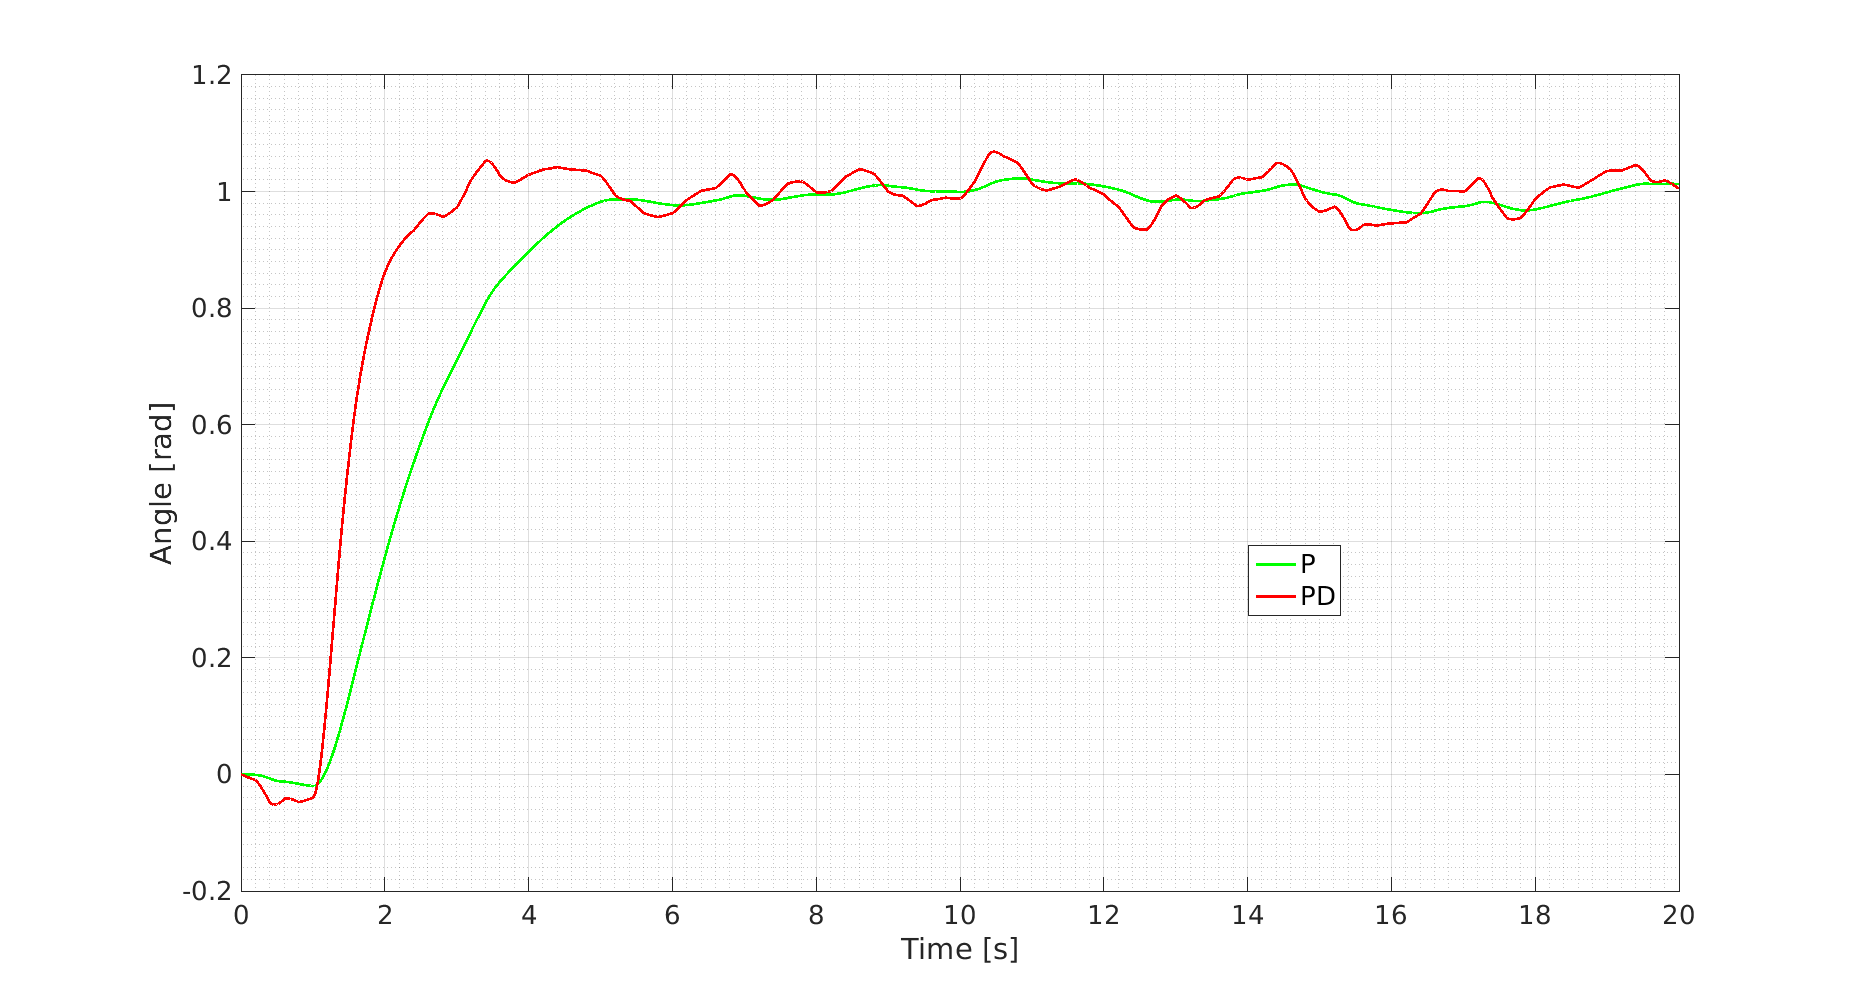
\includegraphics[scale=0.18]{../report/figures/PD_noise.png}
      \end{figure}
  
  \end{block}
\end{frame}

%%% CONTROLLER
%
%
%%Tuning Method
%\begin{frame}{Controller}{Tuning Methods}
%  \begin{block}{PID Simulink Box}
%
%
%	  \begin{itemize}
%	  	\item Weakness of Good Gain Method:
%	  		  \begin{itemize}
%	  	\item Time consuming
%	  	\item Uncertainties of the different steps
%	  \end{itemize}
%	  \item Advantages of PID Simulink Box
%	  \begin{itemize}
%	  	\item Automatic tuning tool
%	  	\item Include N term which avoids a "pure derivative" that reacts easily to noises
%	  \end{itemize}
%	  \end{itemize}
%  
%  \end{block}
%\end{frame}



%%Controller
%\begin{frame}{Controller}{Different controllers}
%  \begin{block}{Different controllers:}
%
%	  \begin{itemize}
%	  	\item PID control
%	 	\begin{itemize}
%	  	\item Proportional
%	  	\item Derivative
%	  	\item Integral
%	  	\item Combination of them
%	  \end{itemize}
%	  \end{itemize}
%
%
% 	  \begin{figure}
%        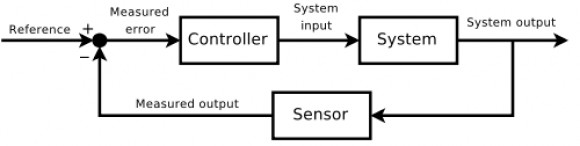
\includegraphics[scale=0.40]{../report/figures/control-theory-chart.jpg}
%      \end{figure} 
%  \end{block}
%\end{frame}
%%
%%Controller P
%\begin{frame}{Controller}{Different controllers}
%  \begin{block}{Proportional Term}
%
%	  \begin{itemize}
%	  	\item Output proportional to the error
%	  \end{itemize}
%
%	  \begin{figure}
%        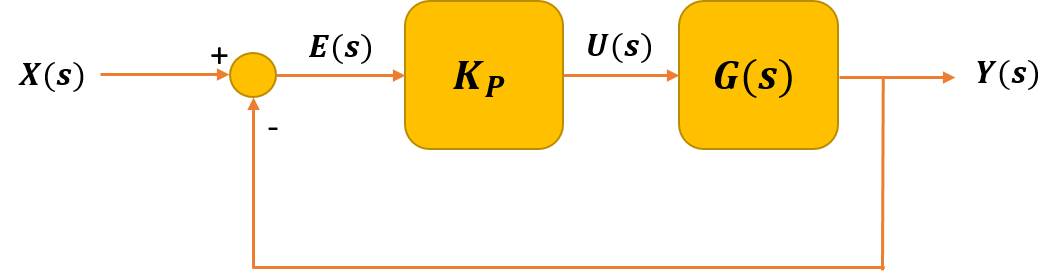
\includegraphics[scale=0.26]{../report/figures/propor_controller.png}
%      \end{figure}
%  
%  \end{block}
%\end{frame}

%%Controller I
%\begin{frame}{Controller}{Different controllers}
%  \begin{block}{Integral Term}
%
%	  \begin{itemize}
%	  	\item Sums the error term over time
%	  	\item No steady state error
%	  	\item Cause the present value to overshoot the reference value
%	  \end{itemize}
%
%	  \begin{figure}
%        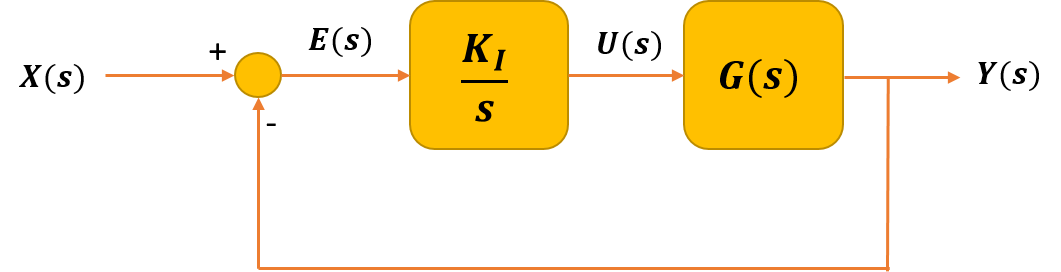
\includegraphics[scale=0.26]{../report/figures/integ_controller.png}
%      \end{figure}
%  
%  \end{block}
%\end{frame}

%%Controller D
%\begin{frame}{Controller}{Different controllers}
%  \begin{block}{Derivative Term}
%
%	  \begin{itemize}
%	  	\item Acts as a brake on the control effort
%	  	\item Highly sensitive to noise
%	  \end{itemize}
%
%	  \begin{figure}
%        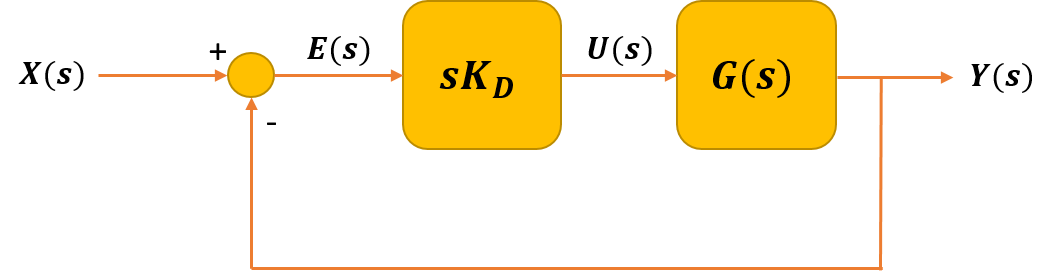
\includegraphics[scale=0.26]{../report/figures/deriv_controller.png}
%      \end{figure}
%  
%  \end{block}
%\end{frame}

%%Controller PI
%\begin{frame}{Controller}{Different controllers}
%  \begin{block}{PI Controller}
%
%	  \begin{itemize}
%	  	\item Eliminate the steady state error
%	  	\item Negative impact on the speed of the response
%	  	\item Should be applied when speed is not an important parameter
%	  \end{itemize}
%
%	  \begin{figure}
%        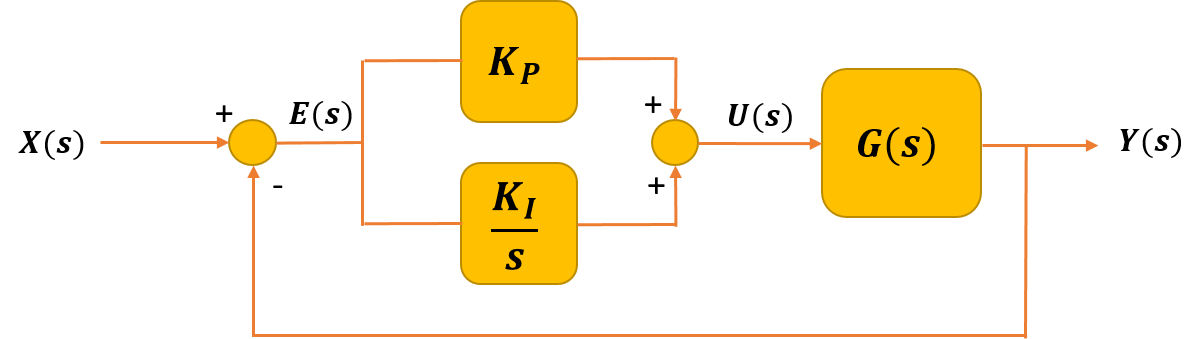
\includegraphics[scale=0.26]{../report/figures/PI_controller.png}
%      \end{figure}
%  
%  \end{block}
%\end{frame}
%
%
%%Controller PD
%\begin{frame}{Controller}{Different controllers}
%  \begin{block}{PD Controller}
%
%	  \begin{itemize}
%	  	\item Why is PD alone good?
%	  \end{itemize}
%
%	  \begin{figure}
%        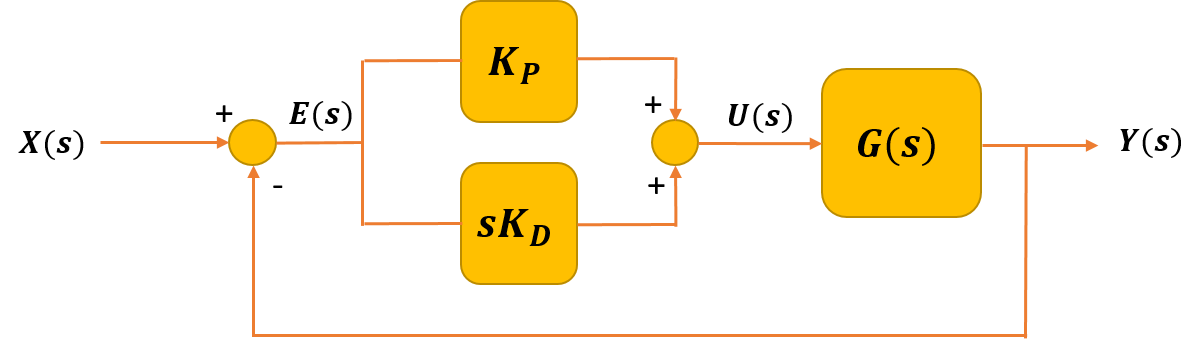
\includegraphics[scale=0.26]{../report/figures/PD_controller.png}
%      \end{figure}
%  
%  \end{block}
%\end{frame}
%
%%Controller PID
%\begin{frame}{Controller}{Different controllers}
%  \begin{block}{PID Controller}
%
%	  \begin{itemize}
%	  	\item Eliminate steady state error
%	  	\item Fast response
%	  	\item Higher stability
%	  	\item (Derivative Term) Reduction of the overshoot and oscillations
%	  \end{itemize}
%
%	  \begin{figure}
%        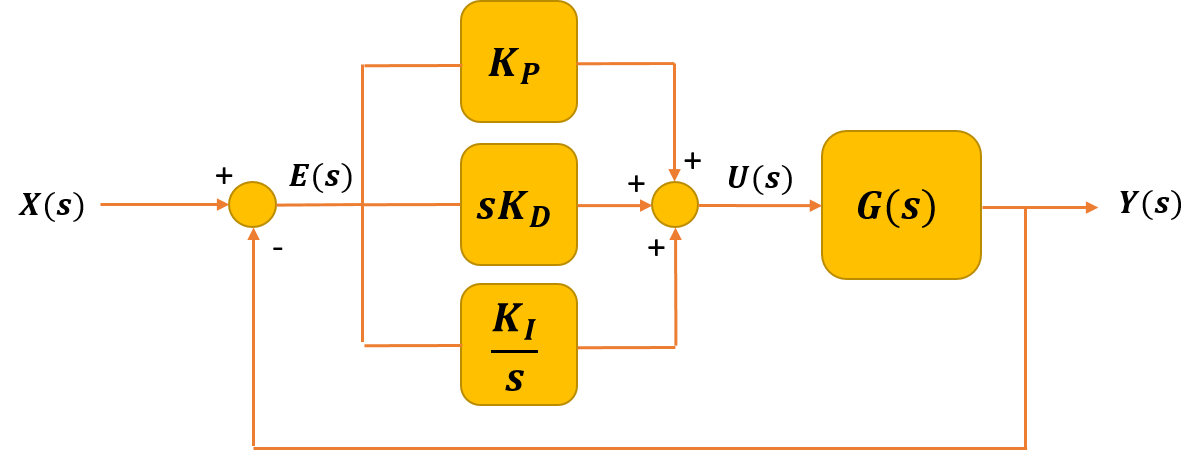
\includegraphics[scale=0.26]{../report/figures/PID_controller.png}
%      \end{figure}
%  
%  \end{block}
%\end{frame}




